  \documentclass{beamer}
\usepackage[utf8]{inputenc}
\usepackage{hyperref}
\usepackage{graphicx}

\usepackage{listings}
\lstset{frame=single,backgroundcolor=\color{lightgray}}
\usetheme{Warsaw}

  \title{Introduction to Linux}
  \author{Pierre Lindenbaum\\@yokofakun\\http://plindenbaum.blogspot.com}\institute{Institut du Thorax. Nantes. France}

\begin{document}

\begin{frame}
\titlepage
\end{frame}



\begin{frame}
\begin{figure}
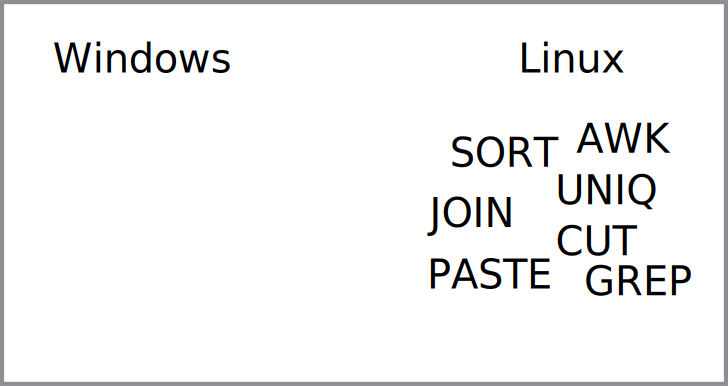
\includegraphics[scale=.5]{linux01.ps}
\end{figure}
\end{frame}

\begin{frame}
\begin{figure}

\includegraphics[scale=.23]{linux02.ps}
\end{figure}
\end{frame}

\begin{frame}
\begin{figure}
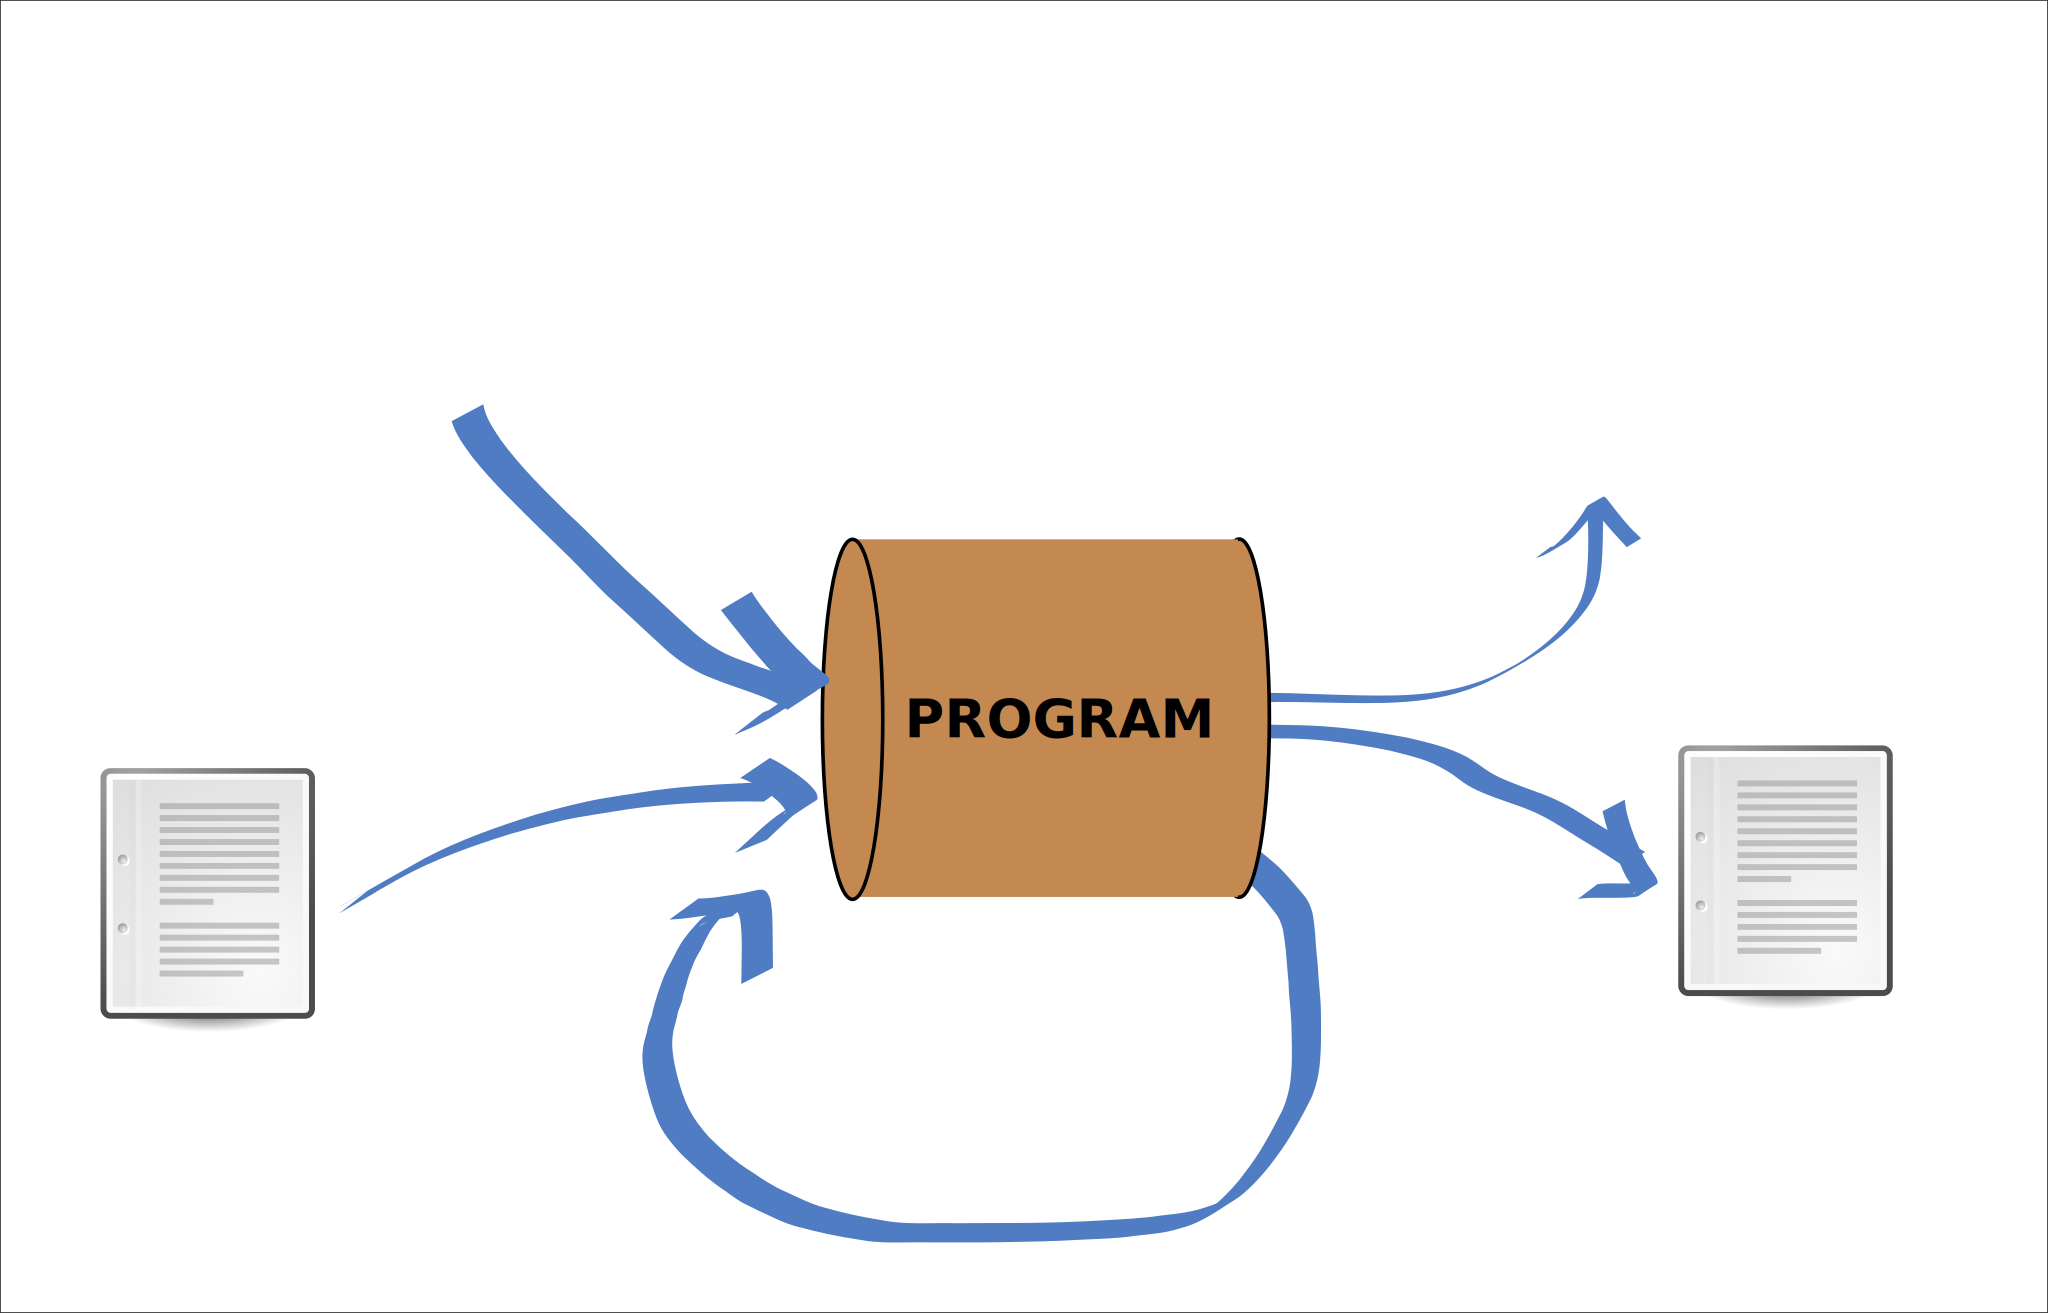
\includegraphics[scale=.15]{linux03.ps}
\end{figure}
\end{frame}


\begin{frame}[fragile]
\begin{lstlisting}[language=bash]
$ programname (options) (files)
\end{lstlisting}
\end{frame}

\begin{frame}[fragile]
\frametitle{Navigation}

where am I ?
\begin{lstlisting}[language=bash]
$ pwd
\end{lstlisting}

Go to directory dir1
\begin{lstlisting}[language=bash]
$ cd dir1
\end{lstlisting}

Go to directory dir1/dir2
\begin{lstlisting}[language=bash]
$ cd dir1/dir2
\end{lstlisting}


Go upper directory
\begin{lstlisting}[language=bash]
$ cd ..
\end{lstlisting}

Go upper directory and then go to dir4
\begin{lstlisting}[language=bash]
$ cd ../dir4
\end{lstlisting}


\end{frame}

\begin{frame}[fragile]
\frametitle{Navigation}

Go to the root
\begin{lstlisting}[language=bash]
$ cd /
\end{lstlisting}

Go to my home
\begin{lstlisting}[language=bash]
$ cd ~
\end{lstlisting}

Go to my previous directory
\begin{lstlisting}[language=bash]
$ cd /
\end{lstlisting}

\end{frame}


\begin{frame}[fragile]
 \begin{center}
    \huge{CASE matters}\\
    \end{center}
\begin{lstlisting}[language=bash]
$ cd dir1
\end{lstlisting}


\begin{lstlisting}[language=bash]
$ cd DIR1
\end{lstlisting}

\end{frame}


\begin{frame}[fragile]
Regular Expression.\\
'?' : The question mark indicates there is zero or one of the preceding element. For example, colou?r matches both "color" and "colour".\\
'*' : The asterisk indicates there is zero or more of the preceding element. For example, ab*c matches "ac", "abc", "abbc", "abbbc", and so on.\\
'+' : The plus sign indicates there is one or more of the preceding element. For example, ab+c matches "abc", "abbc", "abbbc", and so on, but not "ac".\\
(a|b)* denotes the set of all strings.\\
\[ \] : A bracket expression. Matches a single character that is contained within the brackets.\\
\^ 	Matches the starting position within the string.\\
\$ 	Matches the ending position of the string or the position just before a string-ending newline.
\end{frame}


\begin{frame}[fragile]
Escape characters.\\
Cariage Return.
\begin{lstlisting}[language=bash]
\n
\end{lstlisting}
Tabulation.
\begin{lstlisting}[language=bash]
\t
\end{lstlisting}
\end{frame}


\begin{frame}[fragile]
Shell shortcuts.\\
Arrow-up/down: prev/next in history.\\
Ctr-R : Search history.\\
Ctr-A : Begin line.\\
Ctr-E : End line.\\
Ctr-K : Cut line.\\
Ctr-D and tab : insert tabulation.\\
Ctr-D and tab : insert tabulation.\\
Ctr-D (in pipeline): EOF (End Of File).\\
\end{frame}


\begin{frame}[fragile]
 \begin{center}
    \huge{whitespaces matter}\\
    \end{center}
\begin{lstlisting}[language=bash]
$ cd my results
bash: cd: my: No such file or directory
\end{lstlisting}


\begin{lstlisting}[language=bash]
$ cd  "my results"
\end{lstlisting}

\begin{lstlisting}[language=bash]
$ cd my\ results
\end{lstlisting}
  
\end{frame}

\begin{frame}[fragile]
 \begin{center}
    \huge{man}\\
    \end{center}
\begin{lstlisting}[language=bash]
$ man man

MAN(1)                                                               

NAME
       man - an interface to the on-line reference

SYNOPSIS
       man  [-C  file]  [-d]  [-D]  [--warnings[=wa
       [--names-only] [-a] [-u] [--no-subpages] [-P 
       [-X[dpi]] [-Z] [[section] page ...] ...
       man -k [apropos options] regexp ...
       man -K [-w|-W] [-S list] [-i|-I] [--regex] [s
       man -f [whatis options] page ...
       man  -l  [-C  file]  [-d]  [-D] [--warnings[=w
       man -w|-W [-C file] [-d] [-D] page ...
       man -c [-C file] [-d] [-D] page ...

\end{lstlisting}
\end{frame}


\begin{frame}[fragile]
 \begin{center}
    \huge{apropos}\\
    \end{center}
\begin{lstlisting}[language=bash]
$ apropos apropos
apropos (1)          - search the manual page names and 

$ apropos pdf
pdfcrop (1)          - crop pdf files to their minimal 
a2ping (1)           - - convert between PS, EPS and PD
dvipdf (1)           - Convert TeX DVI file to PDF usin
dvipdfm (1)          - Produce PDF files directly from
dvipdft (1)          - create thumbnail images for use 
e2pall (1)           - convert all EPS files in a LaTeX
\end{lstlisting}
\end{frame}

\begin{frame}[fragile]
 \begin{center}
    \huge{pwd}\\
    \end{center}
\begin{lstlisting}[language=bash]
$ pwd
/home/lindenb/src/courses/about.linux
\end{lstlisting}
\end{frame}

\begin{frame}[fragile]
 \begin{center}
    \huge{mkdir}\\
    \end{center}
\begin{lstlisting}[language=bash]
$ mkdir DIR1
$ mkdir DIR1/DIR2
$ mkdir -p DIR1/DIR3/DIR3
\end{lstlisting}
\end{frame}

\begin{frame}[fragile]
 \begin{center}
    \huge{ls}\\
    \end{center}
\begin{lstlisting}[language=bash]
$ ls
$ ls -l
$ ls -la
$ ls -la /home/
\end{lstlisting}
\end{frame}


\begin{frame}[fragile]
 \begin{center}
    \huge{echo}\\
    \end{center}
\begin{lstlisting}[language=bash]
$ echo "ABCD"
$ echo -n "ABCD"
$ echo -e "A\tB\nCD"
\end{lstlisting}
\end{frame}

\begin{frame}[fragile]
 \begin{center}
    \huge{'file'}\\
     	Determine what type of data is within a file.\\
    \end{center}
\begin{lstlisting}[language=bash]
$ file ~/jeter.vcf.gz ~/Documents/2011028.odp
/home/lindenb/jeter.vcf.gz:          gzip compressed data, extra field
/home/lindenb/Documents/2011028.odp: OpenDocument Presentation
\end{lstlisting}
\end{frame}


\begin{frame}[fragile]
 \begin{center}
    \huge{'tr'}\\
     	translate or delete characters.\\
    \end{center}
\begin{lstlisting}[language=bash]
$ echo "AAAAAAABCD" | tr "A" "a"
aaaaaaaBCD

$ echo "AAAAAAABCD" | tr -s "A" 
ABCD

$ echo "AAAAAAABCD" | tr -d "A" 
BCD
\end{lstlisting}
\end{frame}

\begin{frame}[fragile]
 \begin{center}
    \huge{rm}\\
    \end{center}
\begin{lstlisting}[language=bash]
$ rm file1.txt file2.txt
$ rm -r DIR1/file1.txt
$ rm -i DIR1/file1.txt
$ rm -f DIR1/file1.txt
\end{lstlisting}
\end{frame}



\begin{frame}[fragile]
 \begin{center}
    \huge{rmdir}\\
    \end{center}
\begin{lstlisting}[language=bash]
$ rmdir DIR1
\end{lstlisting}
\end{frame}

\begin{frame}[fragile]
 \begin{center}
    \huge{mv}\\
    \end{center}
\begin{lstlisting}[language=bash]
$ mv DIR1/file1.txt DIR2/
$ mv olname.txt newname.txt
\end{lstlisting}
\end{frame}


\begin{frame}[fragile]
 \begin{center}
    \huge{cp}\\
    \end{center}
\begin{lstlisting}[language=bash]
$ cp olname.txt newname.txt
\end{lstlisting}
\end{frame}



\begin{frame}[fragile]
 \begin{center}
    \huge{more}\\
    \end{center}
\begin{lstlisting}[language=bash]
$ more file1.txt file2.txt
\end{lstlisting}
\end{frame}





\begin{frame}[fragile]
 \begin{center}
    \huge{cat}\\
    \end{center}
\begin{lstlisting}[language=bash]
$ cat file1.txt file2.txt
$ cat -n file1.txt
\end{lstlisting}
\end{frame}


\begin{frame}[fragile]
 \begin{center}
    \huge{head}\\
     output the first part of files.\\
    \end{center}
\begin{lstlisting}[language=bash]
$ head file1.txt
$ head -n 100 file1.txt
\end{lstlisting}
\end{frame}


\begin{frame}[fragile]
 \begin{center}
    \huge{tail}\\
     output the last part of files.\\
    \end{center}
\begin{lstlisting}[language=bash]
$ head file1.txt
$ head -n 100 file1.txt
\end{lstlisting}
\end{frame}



\begin{frame}[fragile]
 \begin{center}
    \huge{grep}\\
    \end{center}
\begin{lstlisting}[language=bash]
$ grep Gene1 genes.txt
$ grep -v Gene1 genes.txt
$ grep -i Gene1 genes.txt
$ grep -E '(Gene1|Protein1)' genes.txt
\end{lstlisting}
\end{frame}


\begin{frame}[fragile]
 \begin{center}
    \huge{cut}\\
    \end{center}
\begin{lstlisting}[language=bash]
$ cut -d '	' -f1,2,4-10 file1
$ cut -c1-10 file1
\end{lstlisting}
\end{frame}

\begin{frame}[fragile]
 \begin{center}
    \huge{sort}\\
    \end{center}
\begin{lstlisting}[language=bash]

\end{lstlisting}
\end{frame}


\begin{frame}[fragile]
 \begin{center}
    \huge{uniq}\\
    \end{center}
\begin{lstlisting}[language=bash]

\end{lstlisting}
\end{frame}


\begin{frame}[fragile]
 \begin{center}
    \huge{wc}\\
    \end{center}
\begin{lstlisting}[language=bash]

\end{lstlisting}
\end{frame}


\begin{frame}[fragile]
 \begin{center}
    \huge{awk for filtering}\\
    \end{center}
\begin{lstlisting}[language=bash]
awk -F '	' '($1=="chr1" && int($2)>10 && int($2)<100)' file.vcf
\end{lstlisting}
\end{frame}

\begin{frame}[fragile]
 \begin{center}
    \huge{join}\\
    \end{center}
\begin{lstlisting}[language=bash]
$ join -t '	' -1 1 -2 1 file1.txt file2.txt
\end{lstlisting}
\end{frame}

\begin{frame}[fragile]
 \begin{center}
    \huge{comm}\\
    \end{center}
\begin{lstlisting}[language=bash]
$ comm file1.txt file2.txt
$ comm -12 file1.txt file2.txt
\end{lstlisting}
\end{frame}


\begin{frame}[fragile]
 \begin{center}
    \huge{gzip , gunzip}\\
    \end{center}
\begin{lstlisting}[language=bash]
$ gzip file1.txt
$ gunzip -c file1.txt.gz
$ gunzip  file1.txt
\end{lstlisting}
\end{frame}

\begin{frame}[fragile]
\begin{center}
    \huge{sed}\\
\end{center}
Usage:
\begin{lstlisting}[language=make]
sed 's/PATTERN/REPLACEBY/MODIFIER'
\end{lstlisting}
Examples:
\begin{lstlisting}[language=make]
$ echo "chr1 chr2 chr3" | sed 's/chr/CHROM_/'
CHROM_1 chr2 chr3
$ echo "chr1 chr2 chr3" | sed 's/chr/CHROM_/g'
CHROM_1 CHROM_2 CHROM_3
$ echo "chr1 chr2 chr3" | sed 's/Chr/CHROM_/gi'
CHROM_1 CHROM_2 CHROM_3
$ echo "chr1 chr2 chr3" | sed 's/chr/CHROM_/2'
chr1 CHROM_2 chr3
\end{lstlisting}
\end{frame}


\begin{frame}[fragile]
 \begin{center}
    \huge{cmp}\\
    \end{center}
\begin{lstlisting}[language=bash]
$ cmp file1 file2
\end{lstlisting}
\end{frame}

\begin{frame}[fragile]
 \begin{center}
    \huge{diff}\\
    \end{center}
\begin{lstlisting}[language=bash]
$ diff file1 file2
\end{lstlisting}
\end{frame}

\begin{frame}[fragile]
 \begin{center}
    \huge{find}\\
    \end{center}
\begin{lstlisting}[language=bash]
$ find /path1 /path2/dir2 -name "*.vcf.gz"
\end{lstlisting}
\end{frame}

\begin{frame}[fragile]
 \begin{center}
    \huge{paste}\\
    \end{center}
\begin{lstlisting}[language=bash]
$ paste file1 file2 file3 file4
\end{lstlisting}
\end{frame}

\begin{frame}[fragile]
 \begin{center}
    \huge{curl}\\
    \end{center}
\begin{lstlisting}[language=bash]
$  curl "ftp://ftp.1000genomes.ebi.ac.uk/vol1/ftp/release/20110521/ALL.wgs.phase1_release_v3.20101123.snps_indels_sv.sites.vcf.gz" |\
   gunzip -c | head
   
##fileformat=VCFv4.1
##INFO=<ID=LDAF,Number=1,Type=Float,Description="MLE Allele Frequency Accounting for LD">
##INFO=<ID=AVGPOST,Number=1,Type=Float,Description="Average posterior probability from MaCH/Thunder">
##INFO=<ID=RSQ,Number=1,Type=Float,Description="Genotype imputation quality from MaCH/Thunder">
##INFO=<ID=ERATE,Number=1,Type=Float,Description="Per-marker Mutation rate from MaCH/Thunder">
##INFO=<ID=THETA,Number=1,Type=Float,Description="Per-marker Transition rate from MaCH/Thunder">
##INFO=<ID=CIEND,Number=2,Type=Integer,Description="Confidence interval around END for imprecise variants">
##INFO=<ID=CIPOS,Number=2,Type=Integer,Description="Confidence interval around POS for imprecise variants">
##INFO=<ID=END,Number=1,Type=Integer,Description="End position of the variant described in this record">
##INFO=<ID=HOMLEN,Number=.,Type=Integer,Description="Length of base pair identical micro-homology at event breakpoints">
\end{lstlisting}
\end{frame}


\begin{frame}[fragile]
 \begin{center}
    \huge{bash script}\\
    \end{center}
\begin{lstlisting}[language=bash]
#!/bin/bash
echo "Hello " > hello.txt
echo "World" > world.txt
cat hello.txt world.txt > hellodworld.txt
\end{lstlisting}
\end{frame}

\begin{frame}[fragile]
 \begin{center}
    \huge{make}\\
    \end{center}
\begin{lstlisting}[language=make]
all: hellodworld.txt
        cat $<
hellodworld.txt: hello.txt world.txt
        cat $^ > $@
hello.txt:
        echo "Hello " > $@
world.txt:
        echo "World" > $@
clean:
        rm -f hellodworld.txt  hello.txt world.txt
\end{lstlisting}
\end{frame}



\end{document}

